\documentclass{mimosis}

\usepackage{metalogo}
\usepackage{xargs}                      % Use more than one optional parameter in a new commands
\usepackage{indentfirst}
%
\usepackage[colorinlistoftodos,prependcaption,textsize=tiny]{todonotes}
\newcommandx{\unsure}[2][1=]{\todo[linecolor=red,backgroundcolor=red!25,bordercolor=red,#1]{#2}}
\newcommandx{\change}[2][1=]{\todo[linecolor=blue,backgroundcolor=blue!25,bordercolor=blue,#1]{#2}}

\newcommandx{\info}[2][1=]{\todo[linecolor=OliveGreen,backgroundcolor=OliveGreen!25,bordercolor=OliveGreen,#1]{#2}}
\newcommandx{\improvement}[2][1=]{\todo[linecolor=Plum,backgroundcolor=Plum!25,bordercolor=Plum,#1]{#2}}
\newcommandx{\thiswillnotshow}[2][1=]{\todo[disable,#2]{#1}}
%

\usepackage{float}
\usepackage{geometry}
\usepackage{babel}
\graphicspath{ {./img/} }

\newcommand{\alphabet}{%
  abcdefghijklmnopqrstuvwxyz%
}
\newlength{\textW}
\setlength{\textW}{\widthof{\alphabet}* \real{2.5}}
\geometry{textwidth=\textW,}
\newcommand{\myref}[2]{\hyperref[#2]{#1~\ref*{#2}}}
%%%%%%%%%%%%%%%%%%%%%%%%%%%%%%%%%%%%%%%%%%%%%%%%%%%%%%%%%%%%%%%%%%%%%%%%
% Some of my favourite personal adjustments
%%%%%%%%%%%%%%%%%%%%%%%%%%%%%%%%%%%%%%%%%%%%%%%%%%%%%%%%%%%%%%%%%%%%%%%%
%
% These are the adjustments that I consider necessary for typesetting
% a nice thesis. However, they are *not* included in the template, as
% I do not want to force you to use them.

% This ensures that I am able to typeset bold font in table while still aligning the numbers
% correctly.
\usepackage{etoolbox}
\usepackage{listings}

\usepackage[binary-units=true]{siunitx}
\DeclareSIUnit\px{px}

\sisetup{%
  detect-all           = true,
  detect-family        = true,
  detect-mode          = true,
  detect-shape         = true,
  detect-weight        = true,
  detect-inline-weight = math,
}

%%%%%%%%%%%%%%%%%%%%%%%%%%%%%%%%%%%%%%%%%%%%%%%%%%%%%%%%%%%%%%%%%%%%%%%%
% Hyperlinks & bookmarks
%%%%%%%%%%%%%%%%%%%%%%%%%%%%%%%%%%%%%%%%%%%%%%%%%%%%%%%%%%%%%%%%%%%%%%%%

\usepackage[%
  colorlinks = true,
  citecolor  = OliveGreen,
  linkcolor  = Mahogany,
  urlcolor   = RoyalBlue,
  unicode,
  ]{hyperref}


\newcommand{\smallquote}[1]{
    \begin{center}
        \begin{minipage}{0.5\textwidth}
            \begin{small}
                #1
            \end{small}
        \end{minipage}
        \vspace{0.5cm}
    \end{center}
}

\usepackage{bookmark}

\usepackage[all]{nowidow}

%%%%%%%%%%%%%%%%%%%%%%%%%%%%%%%%%%%%%%%%%%%%%%%%%%%%%%%%%%%%%%%%%%%%%%%%
% Bibliography
%%%%%%%%%%%%%%%%%%%%%%%%%%%%%%%%%%%%%%%%%%%%%%%%%%%%%%%%%%%%%%%%%%%%%%%%
%
% I like the bibliography to be extremely plain, showing only a numeric
% identifier and citing everything in simple brackets. The first names,
% if present, will be initialized. DOIs and URLs will be preserved.

\usepackage[%
  autocite     = plain,
  backend      = biber,
  doi          = true,
  url          = true,
  giveninits   = true,
  hyperref     = true,
  maxbibnames  = 99,
  maxcitenames = 99,
  sortcites    = true,
  style        = iso-numeric,
  ]{biblatex}

%%%%%%%%%%%%%%%%%%%%%%%%%%%%%%%%%%%%%%%%%%%%%%%%%%%%%%%%%%%%%%%%%%%%%%%%
% Some adjustments to make the bibliography more clean
%%%%%%%%%%%%%%%%%%%%%%%%%%%%%%%%%%%%%%%%%%%%%%%%%%%%%%%%%%%%%%%%%%%%%%%%
%
% The subsequent commands do the following:
%  - Removing the month field from the bibliography
%  - Fixing the Oxford commma
%  - Suppress the "in" for journal articles
%  - Remove the parentheses of the year in an article
%  - Delimit volume and issue of an article by a colon ":" instead of
%    a dot ""
%  - Use commas to separate the location of publishers from their name
%  - Remove the abbreviation for technical reports
%  - Display the label of bibliographic entries without brackets in the
%    bibliography
%  - Ensure that DOIs are followed by a non-breakable space
%  - Use hair spaces between initials of authors
%  - Make the font size of citations smaller
%  - Fixing ordinal numbers (1st, 2nd, 3rd, and so) on by using
%    superscripts

% Remove the month field from the bibliography. It does not serve a good
% purpose, I guess. And often, it cannot be used because the journals
% have some crazy issue policies.
\AtEveryBibitem{\clearfield{month}}
\AtEveryCitekey{\clearfield{month}}

% Fixing the Oxford comma. Not sure whether this is the proper solution.
% More information is available under [1] and [2].
%
% [1] http://tex.stackexchange.com/questions/97712/biblatex-apa-style-is-missing-a-comma-in-the-references-why
% [2] http://tex.stackexchange.com/questions/44048/use-et-al-in-biblatex-custom-style
%
\AtBeginBibliography{%
  \renewcommand*{\finalnamedelim}{%
    \ifthenelse{\value{listcount} > 2}{%
      \addcomma
      \addspace
      \bibstring{and}%
    }{%
      \addspace
      \bibstring{and}%
    }
  }
}

% Suppress "in" for journal articles. This is unnecessary in my opinion
% because the journal title is typeset in italics anyway.
\renewbibmacro{in:}{%
  \ifentrytype{article}
  {%
  }%
  % else
  {%
    \printtext{\bibstring{in}\intitlepunct}%
  }%
}

% Remove the parentheses for the year in an article. This removes a lot
% of undesired parentheses in the bibliography, thereby improving the
% readability. Moreover, it makes the look of the bibliography more
% consistent.
\renewbibmacro*{issue+date}{%
  \setunit{\addcomma\space}
    \iffieldundef{issue}
      {\usebibmacro{date}}
      {\printfield{issue}%
       \setunit*{\addspace}%
       \usebibmacro{date}}%
  \newunit}

% Delimit the volume and the number of an article by a colon instead of
% by a dot, which I consider to be more readable.
\renewbibmacro*{volume+number+eid}{%
  \printfield{volume}%
  \setunit*{\addcolon}%
  \printfield{number}%
  \setunit{\addcomma\space}%
  \printfield{eid}%
}

% Do not use a colon for the publisher location. Instead, connect
% publisher, location, and date via commas.
\renewbibmacro*{publisher+location+date}{%
  \printlist{publisher}%
  \setunit*{\addcomma\space}%
  \printlist{location}%
  \setunit*{\addcomma\space}%
  \usebibmacro{date}%
  \newunit%
}

% Ditto for other entry types.
\renewbibmacro*{organization+location+date}{%
  \printlist{location}%
  \setunit*{\addcomma\space}%
  \printlist{organization}%
  \setunit*{\addcomma\space}%
  \usebibmacro{date}%
  \newunit%
}

% Display the label of a bibliographic entry in bare style, without any
% brackets. I like this more than the default.
%
% Note that this is *really* the proper and official way of doing this.
\DeclareFieldFormat{labelnumberwidth}{#1\adddot}

% Ensure that DOIs are followed by a non-breakable space.
\DeclareFieldFormat{doi}{%
  \mkbibacro{DOI}\addcolon\addnbspace
    \ifhyperref
      {\href{http://dx.doi.org/#1}{\nolinkurl{#1}}}
      %
      {\nolinkurl{#1}}
}

\DefineBibliographyStrings{english}{
  online = {online}
}

\DefineBibliographyStrings{english}{
  urlalso = {Available from}
}


% Use proper hair spaces between initials as suggested by Bringhurst and
% others.
\renewcommand*\bibinitdelim {\addnbthinspace}
\renewcommand*\bibnamedelima{\addnbthinspace}
\renewcommand*\bibnamedelimb{\addnbthinspace}
\renewcommand*\bibnamedelimi{\addnbthinspace}

% Make the font size of citations smaller. Depending on your selected
% font, you might not need this.
\renewcommand*{\citesetup}{%
  \biburlsetup
  \small
}

\DeclareLanguageMapping{english}{english-mimosis}


\addbibresource{Thesis.bib}

%%%%%%%%%%%%%%%%%%%%%%%%%%%%%%%%%%%%%%%%%%%%%%%%%%%%%%%%%%%%%%%%%%%%%%%%
% Fonts
%%%%%%%%%%%%%%%%%%%%%%%%%%%%%%%%%%%%%%%%%%%%%%%%%%%%%%%%%%%%%%%%%%%%%%%%

\ifxetexorluatex
  \setmainfont{Minion Pro}
\else
  \usepackage[lf]{ebgaramond}
  \usepackage[oldstyle,scale=0.7]{sourcecodepro}
  \singlespacing
\fi

\renewcommand{\th}{\textsuperscript{\textup{th}}\xspace}


\makeindex
\makeglossaries

%%%%%%%%%%%%%%%%%%%%%%%%%%%%%%%%%%%%%%%%%%%%%%%%%%%%%%%%%%%%%%%%%%%%%%%%
% Incipit
%%%%%%%%%%%%%%%%%%%%%%%%%%%%%%%%%%%%%%%%%%%%%%%%%%%%%%%%%%%%%%%%%%%%%%%%

\title{Title of the Bachelors thesis goes here}
\author{Tomáš Jaroš}

% This ensures that the subsequent sections are being included as root
% items in the bookmark structure of your PDF reader.
\begin{document}
\frontmatter
    \begin{titlepage}
  \vspace*{2cm}
  \makeatletter
  \begin{center}
      \begin{LARGE}
          \textsc{Masaryk University}
      \end{LARGE}\\[0.01cm]
      \begin{Large}
          \textsc{Faculty of Informatics\\}
      \end{Large}
      \vspace*{1cm}
      
\includegraphics[width=40mm]{fithesis-fi.pdf}\\
      \vspace*{3cm}
    \begin{Huge}
      \@title
    \end{Huge}\\[1.5cm]
    %
    \begin{Large}
        \textsc{Bachelor's Thesis}
    \end{Large}\\[1.5cm]
    %
    \begin{LARGE}
        \@author
    \end{LARGE}
    %
    \vfill
  \end{center}
  \begin{flushright}
      \begin{large}
        May 2022
      \end{large}
  \end{flushright}
  \makeatother
\end{titlepage}

\newpage
\null
\thispagestyle{empty}
\newpage


    %\chapter*{Declaration}

\noindent
Hereby I declare, that this thesis is my original work, which I
have worked out on my own. All sources, references and literature used or
excerpted during elaboration of this work are properly cited and listed in
complete reference to the due source.

\vspace{1cm}
\begin{flushright}
    Tomáš Jaroš
\end{flushright}
\vfill
\textbf{Advisor:} doc. RNDr. Petr Švenda, Ph.D.

    %\chapter*{Acknowledgements}
\noindent
I want to express my utmost gratitude to my advisor, doc. Petr Švenda, for his professional guidance, patience, and helpful advice he provided me during the preparation of this thesis. I would also like to thank my family for their immense support and encouragement throughout my studies.
    %\chapter*{Abstract}
\noindent


\section*{Keywords}
\noindent
% TODO

    \tableofcontents
    \listoffigures
    \glsaddall
    %\printglossary[type=\acronymtype]
    %\chapter{Introduction}
The Trusted Platform Module is a device designed to enhance the security of computing platforms. Many different vendors produce these devices while adhering to the standardized specifications, which define both the mandatory and the optional components. This results in devices having the required functionality in common, but the optional functionality is left to the device architects to include. Thus the produced devices may vary in functionality and performance because the implementation details vary across different vendors.

The objective of this thesis is to implement a tool for the visualization of data collected from Trusted Platform Modules. The resulting tool should be able to create visualizations for several datasets which report on supported functionality, performance characteristics, and cryptographic properties. The visualizations should also be compatible with datasets that report on similar information collected from different secure devices, the JavaCard smart cards.

The first chapter provides an overview of Trusted Platform Module technology. The second chapter analyses the current state of an existing solution for visualization and describes design decisions behind the tool created as the objective of this thesis. The final chapter  presents the outcome of this thesis, a tool called \texttt{AlgTest pyProcess}.




\mainmatter
  %\chapter{State of the Art}

\section{Trusted Platform Module}
The Trusted Platform Module is a system component used as a cryptographic co-processor. It was developed by and standardized by the Trusted Computing Group (TCG) consortium with the purpose of laying a foundation on which secure systems could be further created and developed. 

\subsection{History}
The first broadly used specification was TPM 1.1b, released in 2003. TPMs released under this specification already provided some essential functions found in modern TPMs consisting of key generation of RSA key pairs, storage, secure authorisation, and device-health attestation. For the sake of assuring privacy, the
use of anonymous identity keys based on certificates was introduced. In order to take advantage of such
functionality, these certificates needed to be provided with the TPM, and any generation of such keys was available only after owner authorisation. To be able to anonymously prove the origin of the keys generated
by TPM, a \texttt{privacy certification authority} was created. The integrity of measurements collected during systems boot sequence is provided by Platform Configuration Registers (PCRs). Both PCRs and identity keys might have been used to prove the health of the system's boot sequence~\cite{arthur2015practical}.


The hardware specification was not standardized in TPM 1.1b. This caused various incompatibilities. The TPMs across different vendors provided differing interfaces, which required different drivers. Pin-outs on the chips were not prescribed by any standard. Additionally, there were no countermeasures against dictionary attacks~\cite{arthur2015practical}.
% Should i also mention DAA ?

While being in development from 2005 to 2009, the TPM 1.2 specification went through numerous releases. Regarding the need to store shipped certificates for TPM's endorsement keys on a hard disk, about 2KB of non-volatile RAM was added. A new design needed to be made to support key migration between different TPMs because the old design of key migration would in TPM 1.12 require users to have TPM owner authorization. The new idea made users able to create migratable keys and then relied on a designated third party that could exclusively migrate such keys. Said keys could also be certified. Thus, they were called Certified Migratable keys. Additionally, an internal timer able to synchronize with the external one was added in 1.12, which has its use when signing data due to timestamps. Version 1.12 required API to provide backward compatibility for 1.1b. This increased the complexity of the new specification. The TPM 1.12 became widely used in x86 personal computers starting 2005 and later in 2008 also in servers~\cite{arthur2015practical}.

One of the factors that contributed to the need for yet another specification after TPM 1.12 was that in 2005, some substantial collision attacks were found against the SHA-1 hash function. Analysis regarding the use of SHA-1 in TPM revealed the attacks not being applicable~\cite{tcg_tpm1.12_sha-1_uses}. Due to the extensive use of SHA-1 in TPM 1.12, the new specification had to permit any hashing algorithm without the need to make any changes to the specification. A so-called \texttt{digest agility}. Another problem was the lack of a symmetric algorithm required in the TPM specification. The use of RSA for encryption of serialized data was impractical because RSA operations are slow. Neither would help support bigger-sized RSA keys because that would cause a higher chip cost, incompatibility issues, and lower performance. That's why it was decided that the following specification would adopt support for symmetric encryption, which is faster and more suitable for encryption of large byte streams. Having this many problems, an overhaul of the specification would be convenient. And the architects of TPM 2.0 took advantage of the situatio~\cite{arthur2015practical}.


\subsection{Features}


\section{Performance analysis}
\subsection{tpm2-algtest}
The \texttt{tpm2-algtest}\footnote{https://github.com/crocs-muni/tpm2-algtest} is a tool for automatic gathering of information about the TPM2 devices \cite{Struk2019thesis}. The tool uses libraries implementing Trusted Computing Group's TPM2 Software Stack\footnote{https://github.com/tpm2-software/tpm2-tss} which allows for simplification of development when programming applications supposed to interact with the TPM. The tool tests for support of specific commands and supporting routines, values of structures defined in the TPM 2.0 specification \cite{tcg_p3_commands, tcg_p4_supproutines, tcg_p2_structures}. Supported cryptographic algorithms are also subject to performance analysis where the time to execute such an algorithm is repeatedly measured and recorded. Additionally, the tool uses the TPM to generate key pairs for RSA and ECC-based algorithms so that they can be further analyzed by various means.
be dodo

  %\include{Sources/Practical}
  %\include{Sources/Analysis}

  \bookmarksetup{startatroot}


  %\chapter{Conclusion}


  %% \appendix
\renewcommand{\thechapter}{A}
\chapter{Usage of AlgTest pyProcess}

\definecolor{codegreen}{rgb}{0,0.6,0}
\definecolor{codegray}{rgb}{0.5,0.5,0.5}
\definecolor{codepurple}{rgb}{0.58,0,0.82}
\definecolor{backcolour}{rgb}{0.95,0.95,0.92}

\lstdefinestyle{mystyle}{
    backgroundcolor=\color{white},   
    commentstyle=\color{codegreen},
    keywordstyle=\color{magenta},
    numberstyle=\tiny\color{codegray},
    stringstyle=\color{codepurple},
    basicstyle=\ttfamily\footnotesize,
    breakatwhitespace=false,         
    breaklines=true,                 
    captionpos=b,                    
    keepspaces=true,                          
    showspaces=false,                
    showstringspaces=false,
    showtabs=false,                  
    tabsize=2
}

\lstset{style=mystyle}

\section{Installation}
After cloning into repository containing \texttt{AlgTest process} tool, it is necessary to install a few dependencies. The project includes a script called \texttt{setup.py} which, when ran installs required packages. It may be convenient to create a Python virtual environment that allows us to install and manage Python project packages locally without unnecessary global installation. It is important to create and source a virtual environment before running the setup script.
\begin{lstlisting}[language=bash]
    $ python -m venv venv
    $ source venv/bin/activate
    $ python setup.py
\end{lstlisting}

\section{Folder structure}
\begin{itemize}
    \item \texttt{algtestprocess}
        \begin{itemize}
            \item \texttt{modules} -- folder containing \texttt{algtestprocess} modules.
                \begin{itemize}
                    \item \texttt{components} -- folder containing reusable code for parts of HTML documents. Each file contains classes, constants related to one component.
                    \item \texttt{pages} -- folder containing files with classes corresponding to generated HTML pages, each page has a separate file containing class which is responsible for page creation.
                    \item \texttt{parser}
                        \begin{itemize}
                            \item \texttt{javacard} -- folder containing parser implementations for JavaCard profiles
                            \item \texttt{tpm} -- folder containing parser implementations for TPM profiles
                        \end{itemize}
                    \item \texttt{config.py} -- file containing classes for choice of algorithms used in specific pages
                    \item \texttt{jcalgtest.py} -- file containing classes for storage of Java Card profiles
                    \item \texttt{tpmalgtest.py} -- file containing classes for storage of TPM profiles
                \end{itemize}
        \end{itemize}
    \item \texttt{setup.py} -- script for installation of dependencies and download of results from their official GitHub repository\footnote{\url{https://github.com/crocs-muni/jcalgtest_results}}
    \item \texttt{process.py} -- main entrypoint for generation of outputs, its usage is described in following section
\end{itemize}

\section{Usage}
The script process.py provides a CLI in the following way:

\begin{itemize}
    \item Set of operations from \texttt{process, all, execution-time, comparative, radar, scalability, similarity, support}. We can select multiple operations; however, \texttt{process} operation needs to be run at least once so that some issues with CSV files are fixed, and JSON outputs are generated for the following operations which use them. In the subsequent runs the \texttt{process} argument is not necessary.
    \item \texttt{-i/-{}-results-dir} A directory with measurement results.
    \item \texttt{-o/-{}-output-dir} Output directory to which the HTML outputs are stored.
\end{itemize}

\begin{lstlisting}[language=bash]
    $ python process.py process all --results-dir ./jcalgtest_results/ --output-dir ./jcalgtest_results/javacard/web
    $ python process.py radar scalability -i ./jcalgtest_results/ -o ./jcalgtest_results/javacard/web
\end{lstlisting}

\renewcommand{\thechapter}{B}
\chapter{Diagrams and Visualizations}\label{appendix:diagrams-visualizations}

\begin{figure}[H]
    \centering
    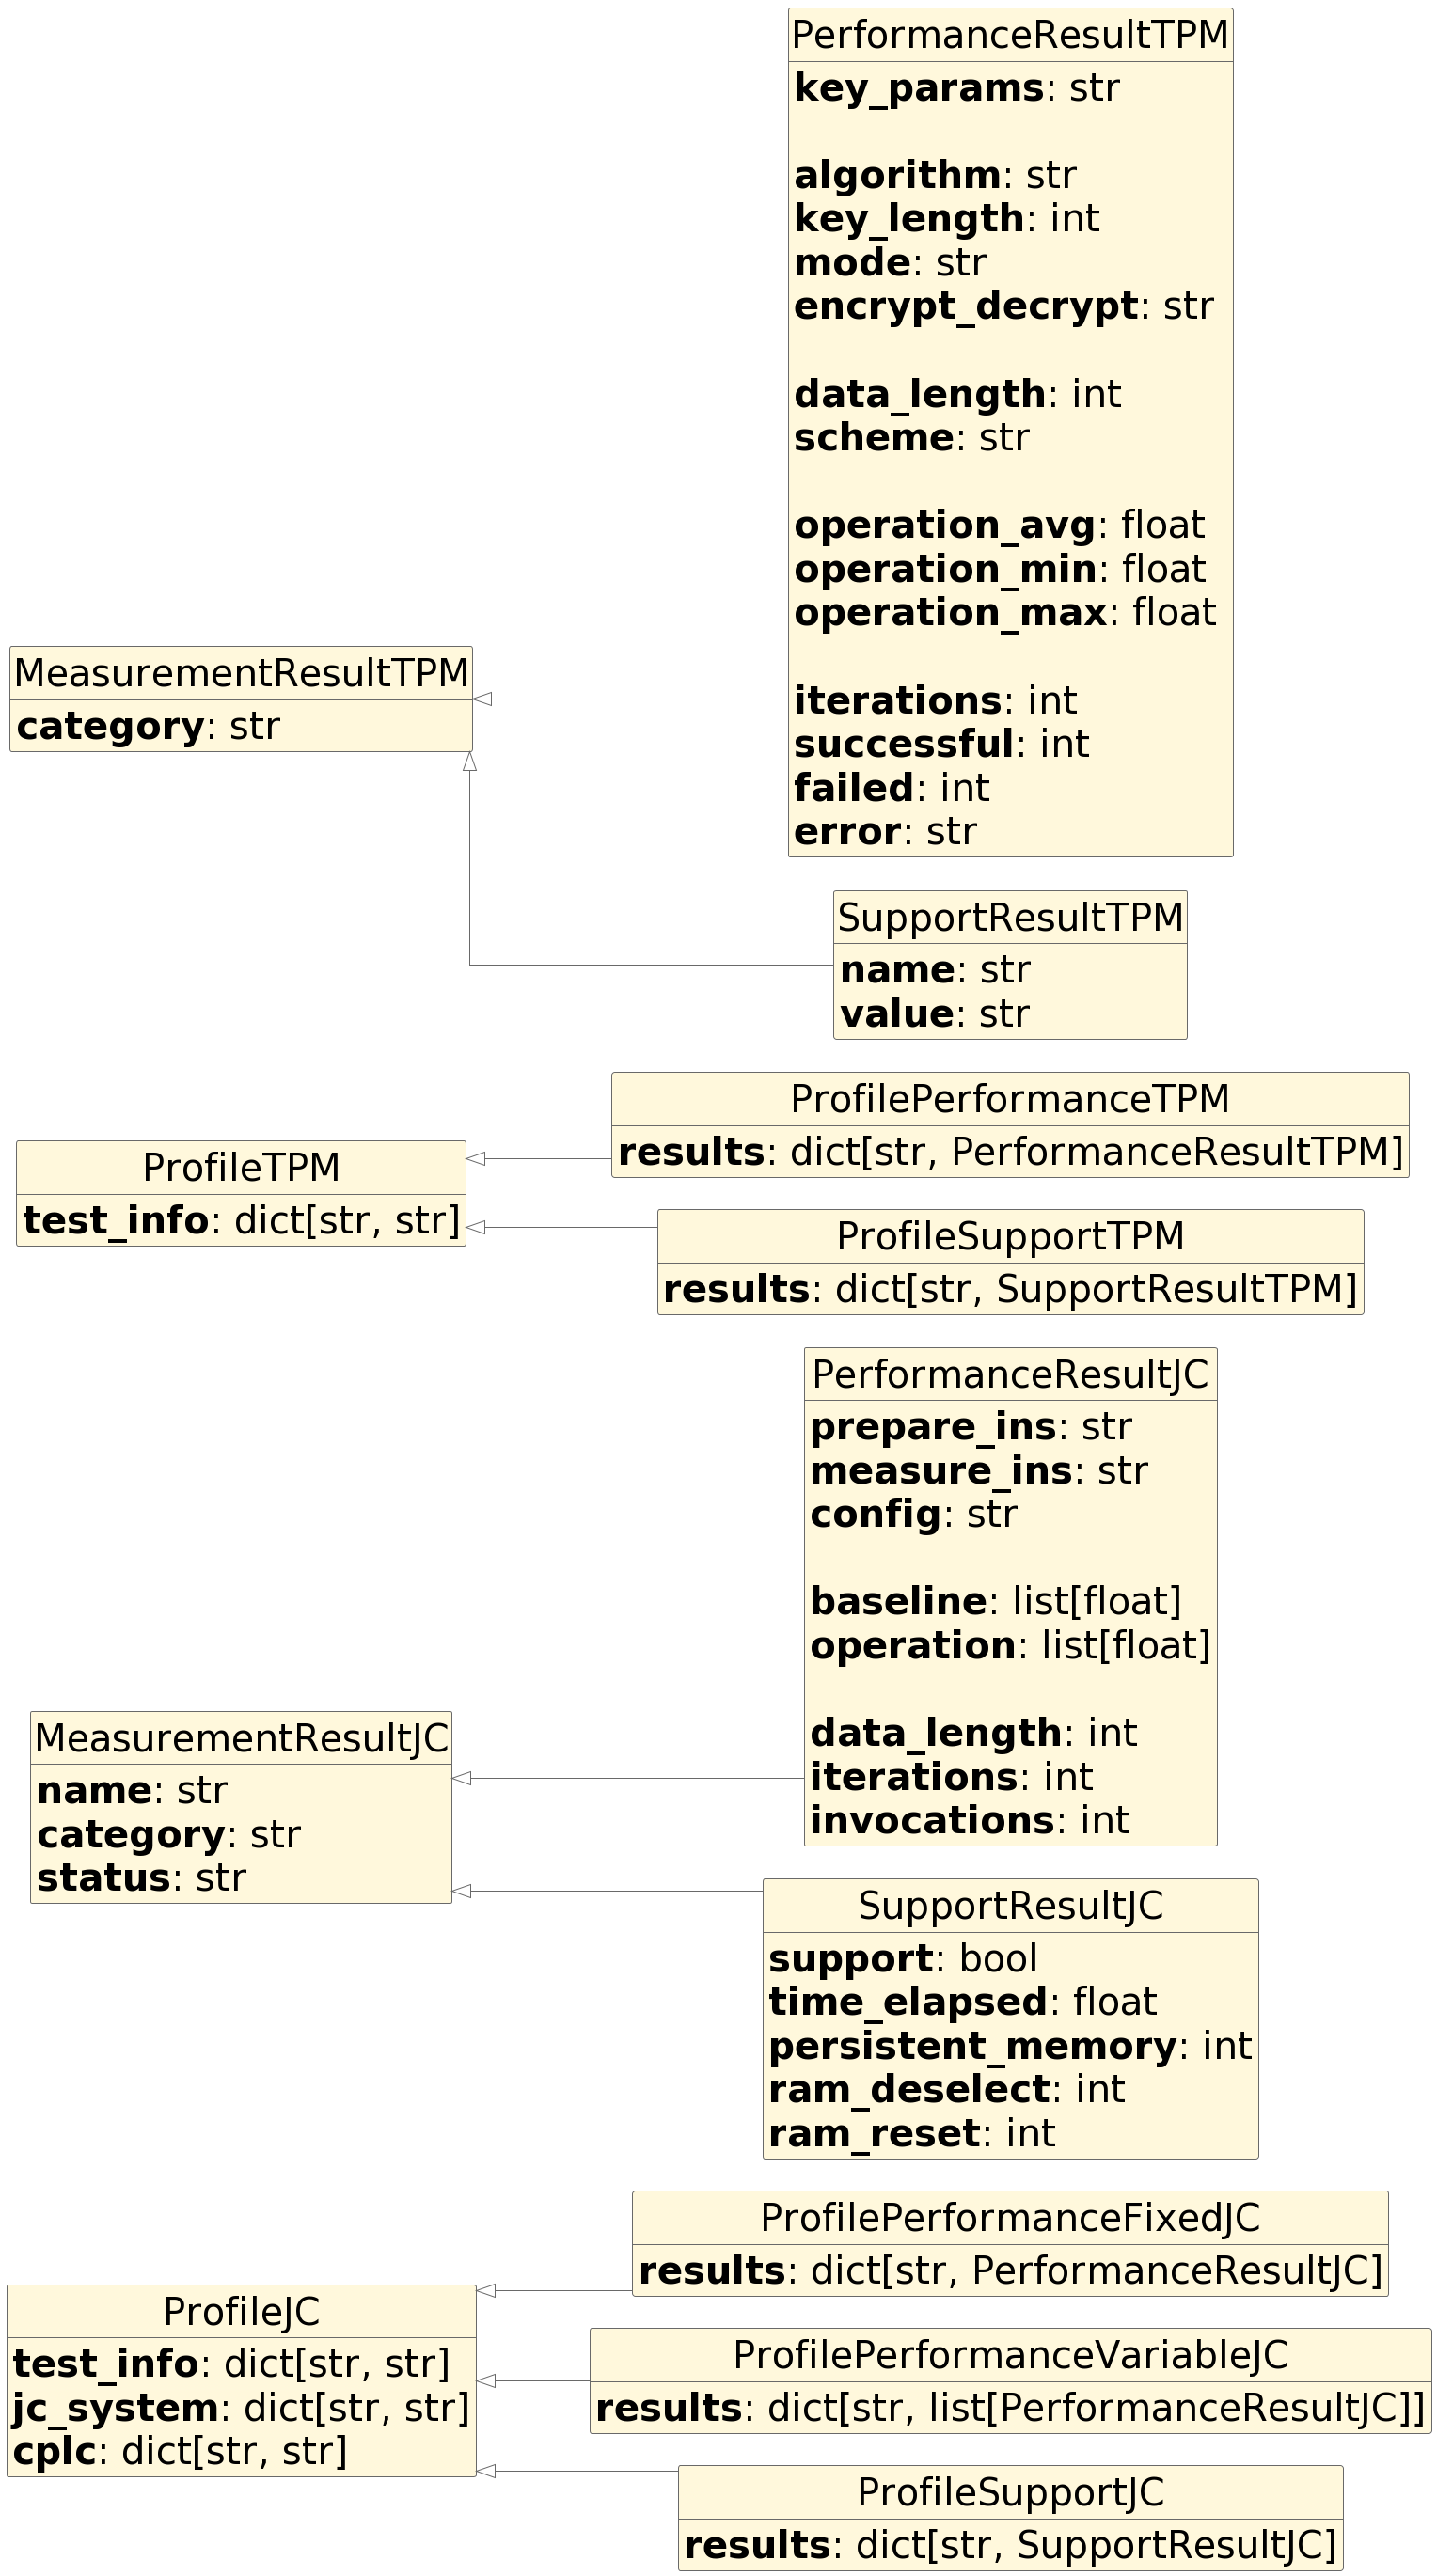
\includegraphics[width=\textwidth,height=\textheight-4.5cm, keepaspectratio]{img/diagrams/object_diagram.png}
    \caption{Diagram of Device profiles}
    \label{fig:dev-profiles-diagram}
\end{figure}

\begin{landscape}
    \begin{figure}[!t]
        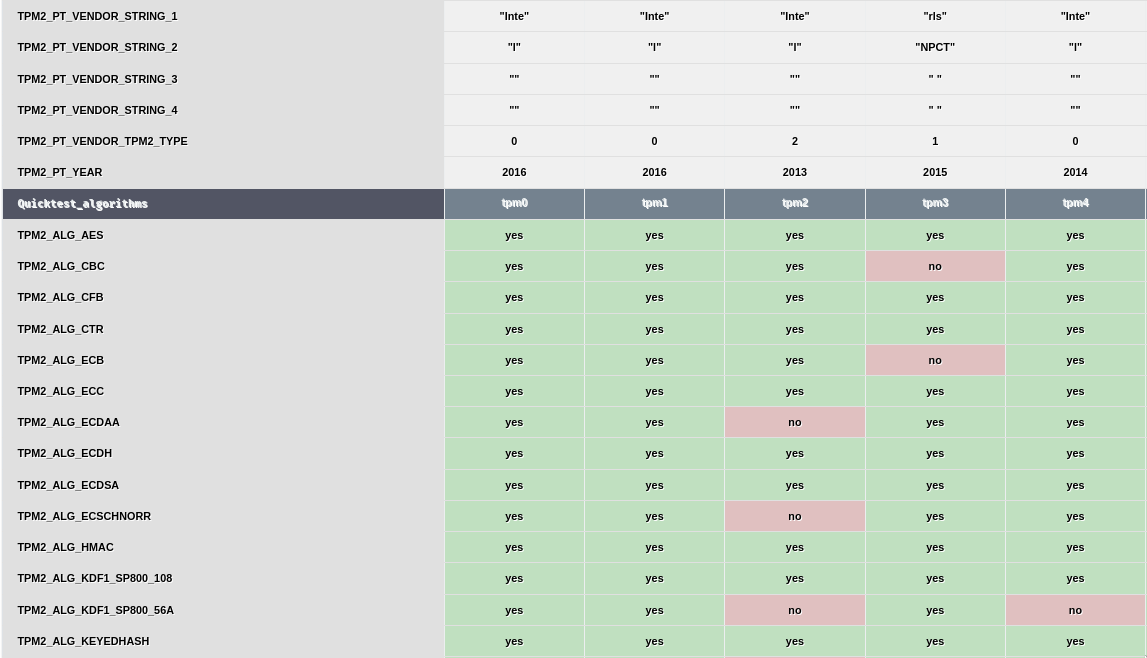
\includegraphics[width=\linewidth, height=\textwidth]{img/visualizations/tpm-support-data.png}
        \caption{An example of a part of Support table visualization for the TPMs}
    \end{figure}
\end{landscape}

\begin{landscape}
    \begin{figure}[!t]
        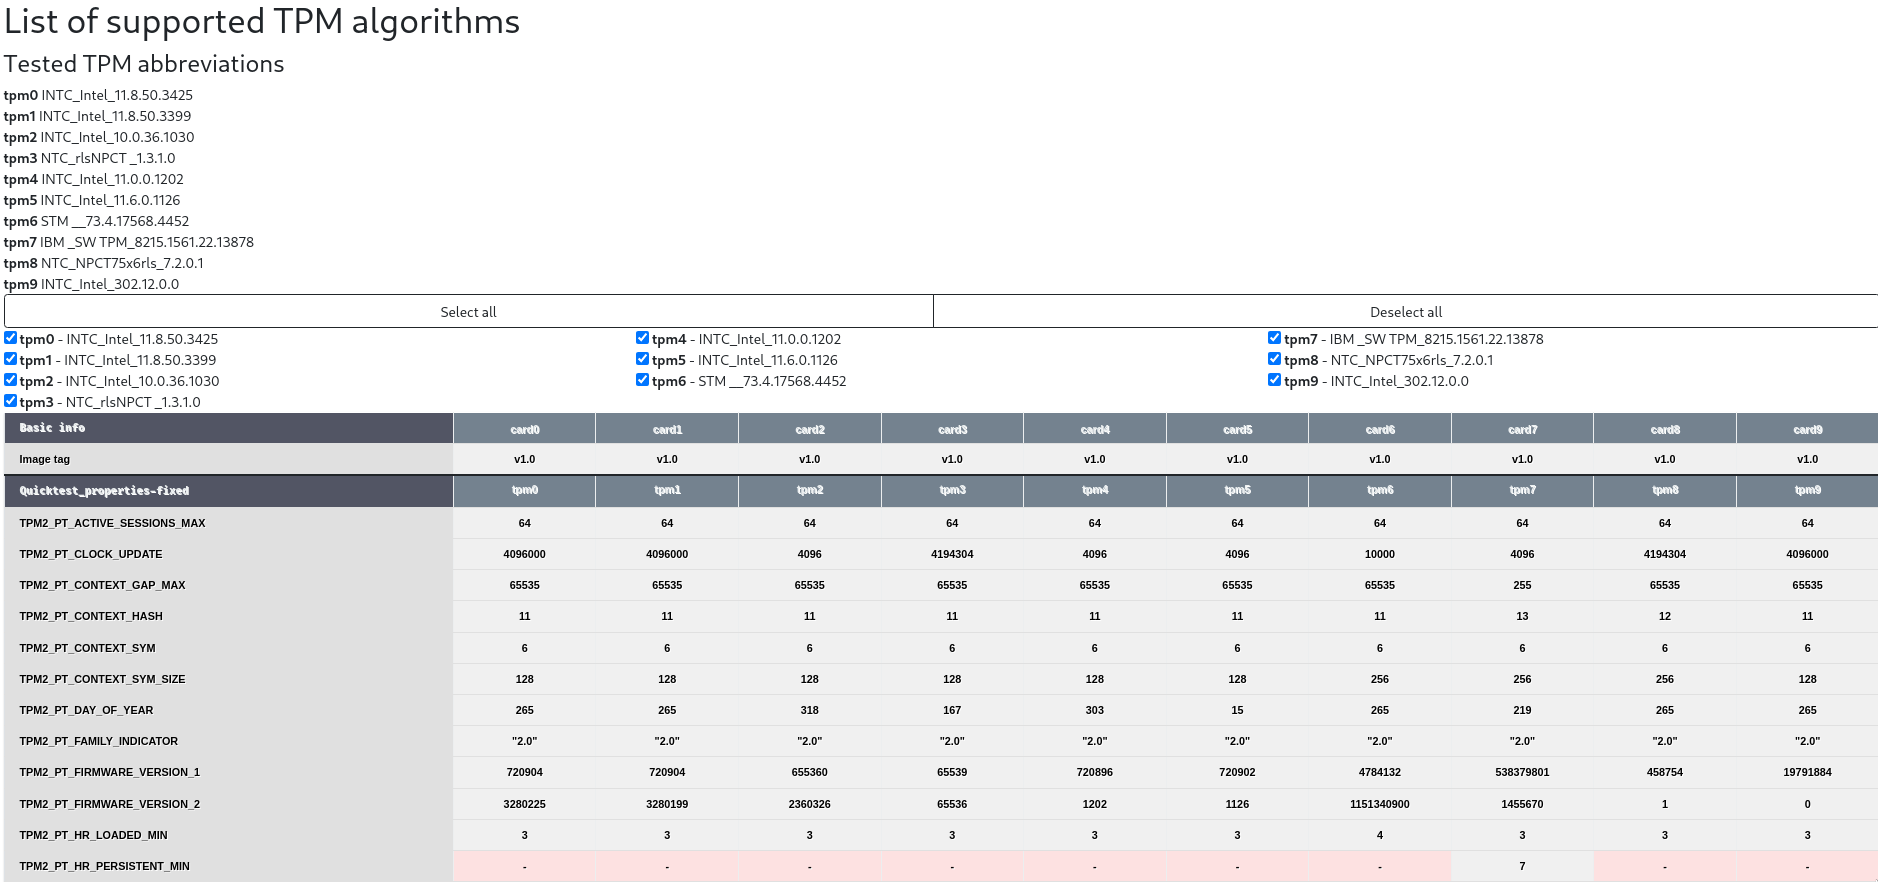
\includegraphics[width=\linewidth, height=\textwidth]{img/visualizations/tpm-support-utility.png}
        \caption{Support tables also contain checkbox utility for filtering the devices}
    \end{figure}
\end{landscape}

\begin{landscape}
    \begin{figure}[!t]
        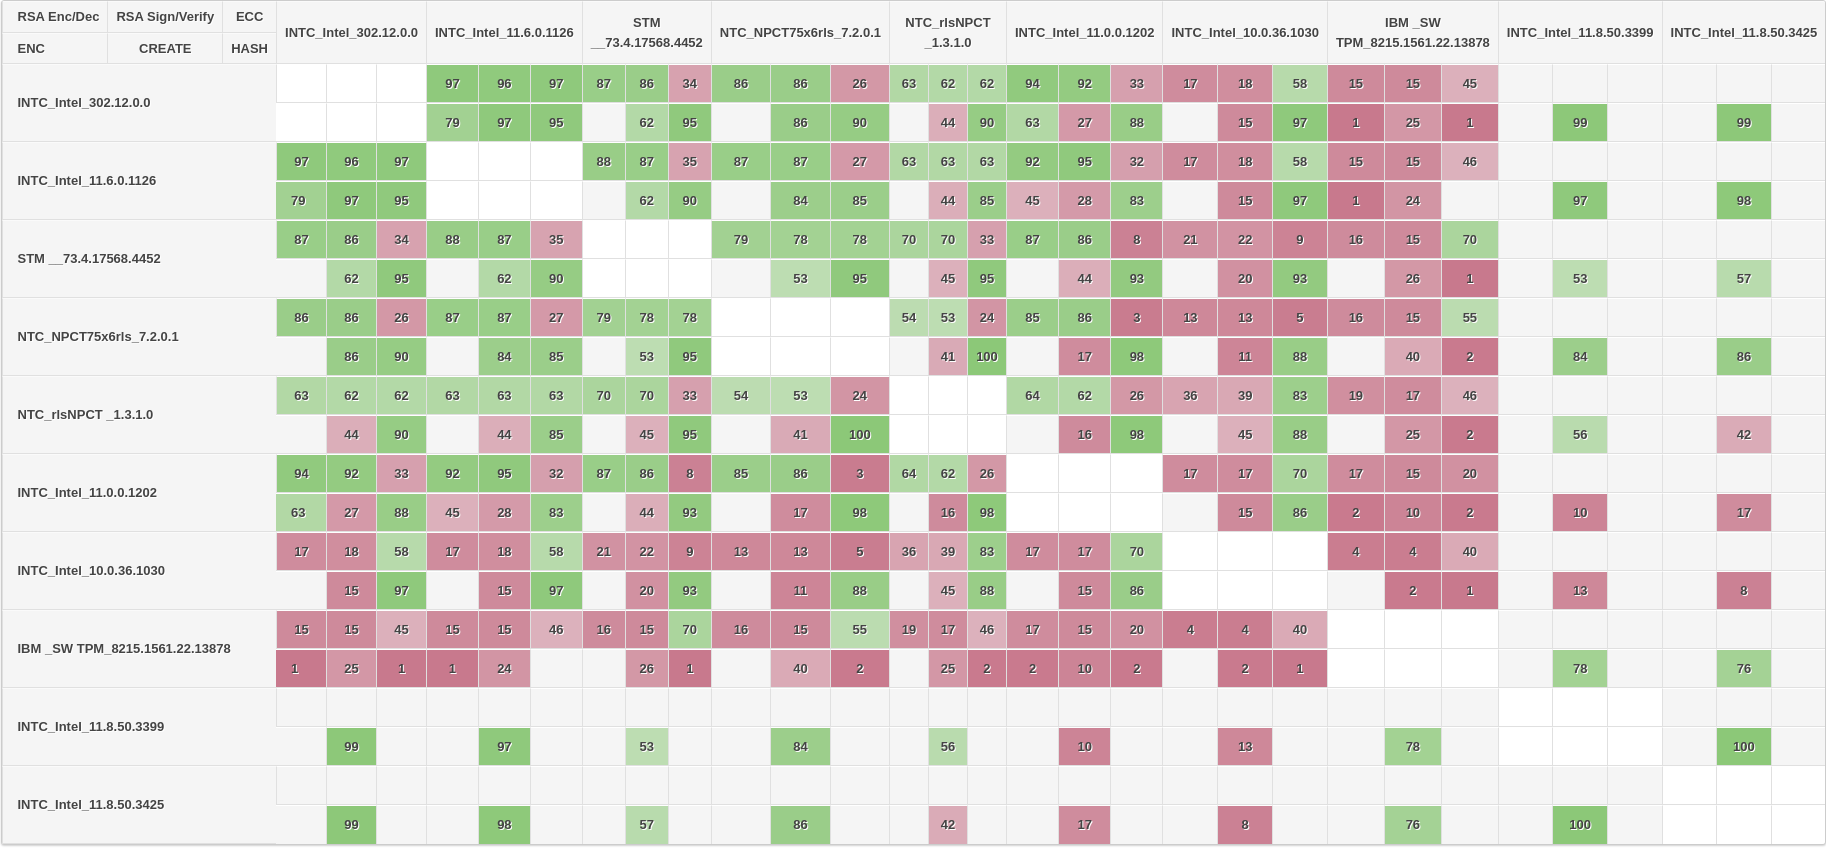
\includegraphics[width=\linewidth, height=\textwidth]{img/visualizations/tpm-similarity.png}
        \caption{Similarity table for TPMs}
    \end{figure}
\end{landscape}

\begin{landscape}
\begin{figure}[!t]
    \centering
    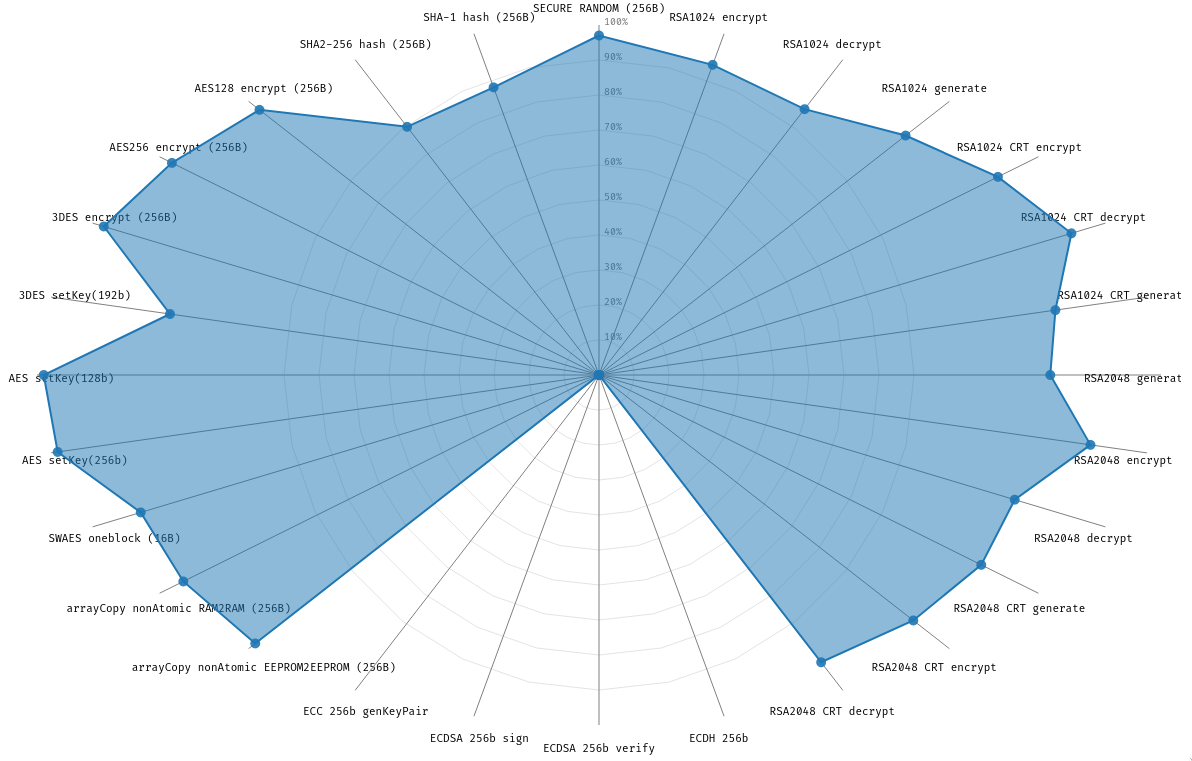
\includegraphics[width=\linewidth]{img/visualizations/JC30M48CR radar graph.png}
    \caption{
    The radar graph of the JC30M48CR smart card. Its performance can be considered excellent, apart from no evident support for algorithms involving Elliptic Curve Cryptography signified by a cut-out at the bottom of the graph.
    }
\end{figure}
\end{landscape}

\begin{landscape}
\begin{figure}[!t]
    \centering
    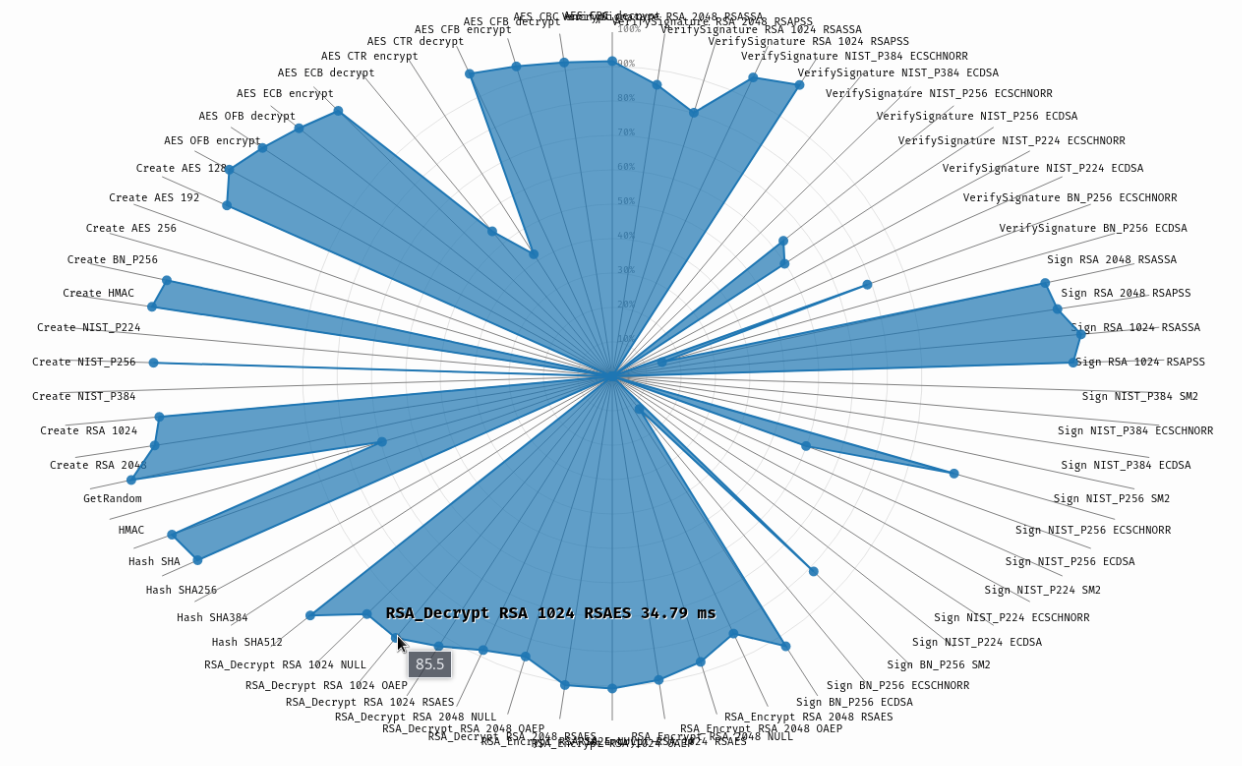
\includegraphics[width=\linewidth]{img/visualizations/INTC_Intel_302.12.0.0 radar graph.png}
    \caption{
    The radar graph of the INTC Intel 302.12.0.0 TPM.
    }
\end{figure}
\end{landscape}
\begin{figure}[H]
    \centering
    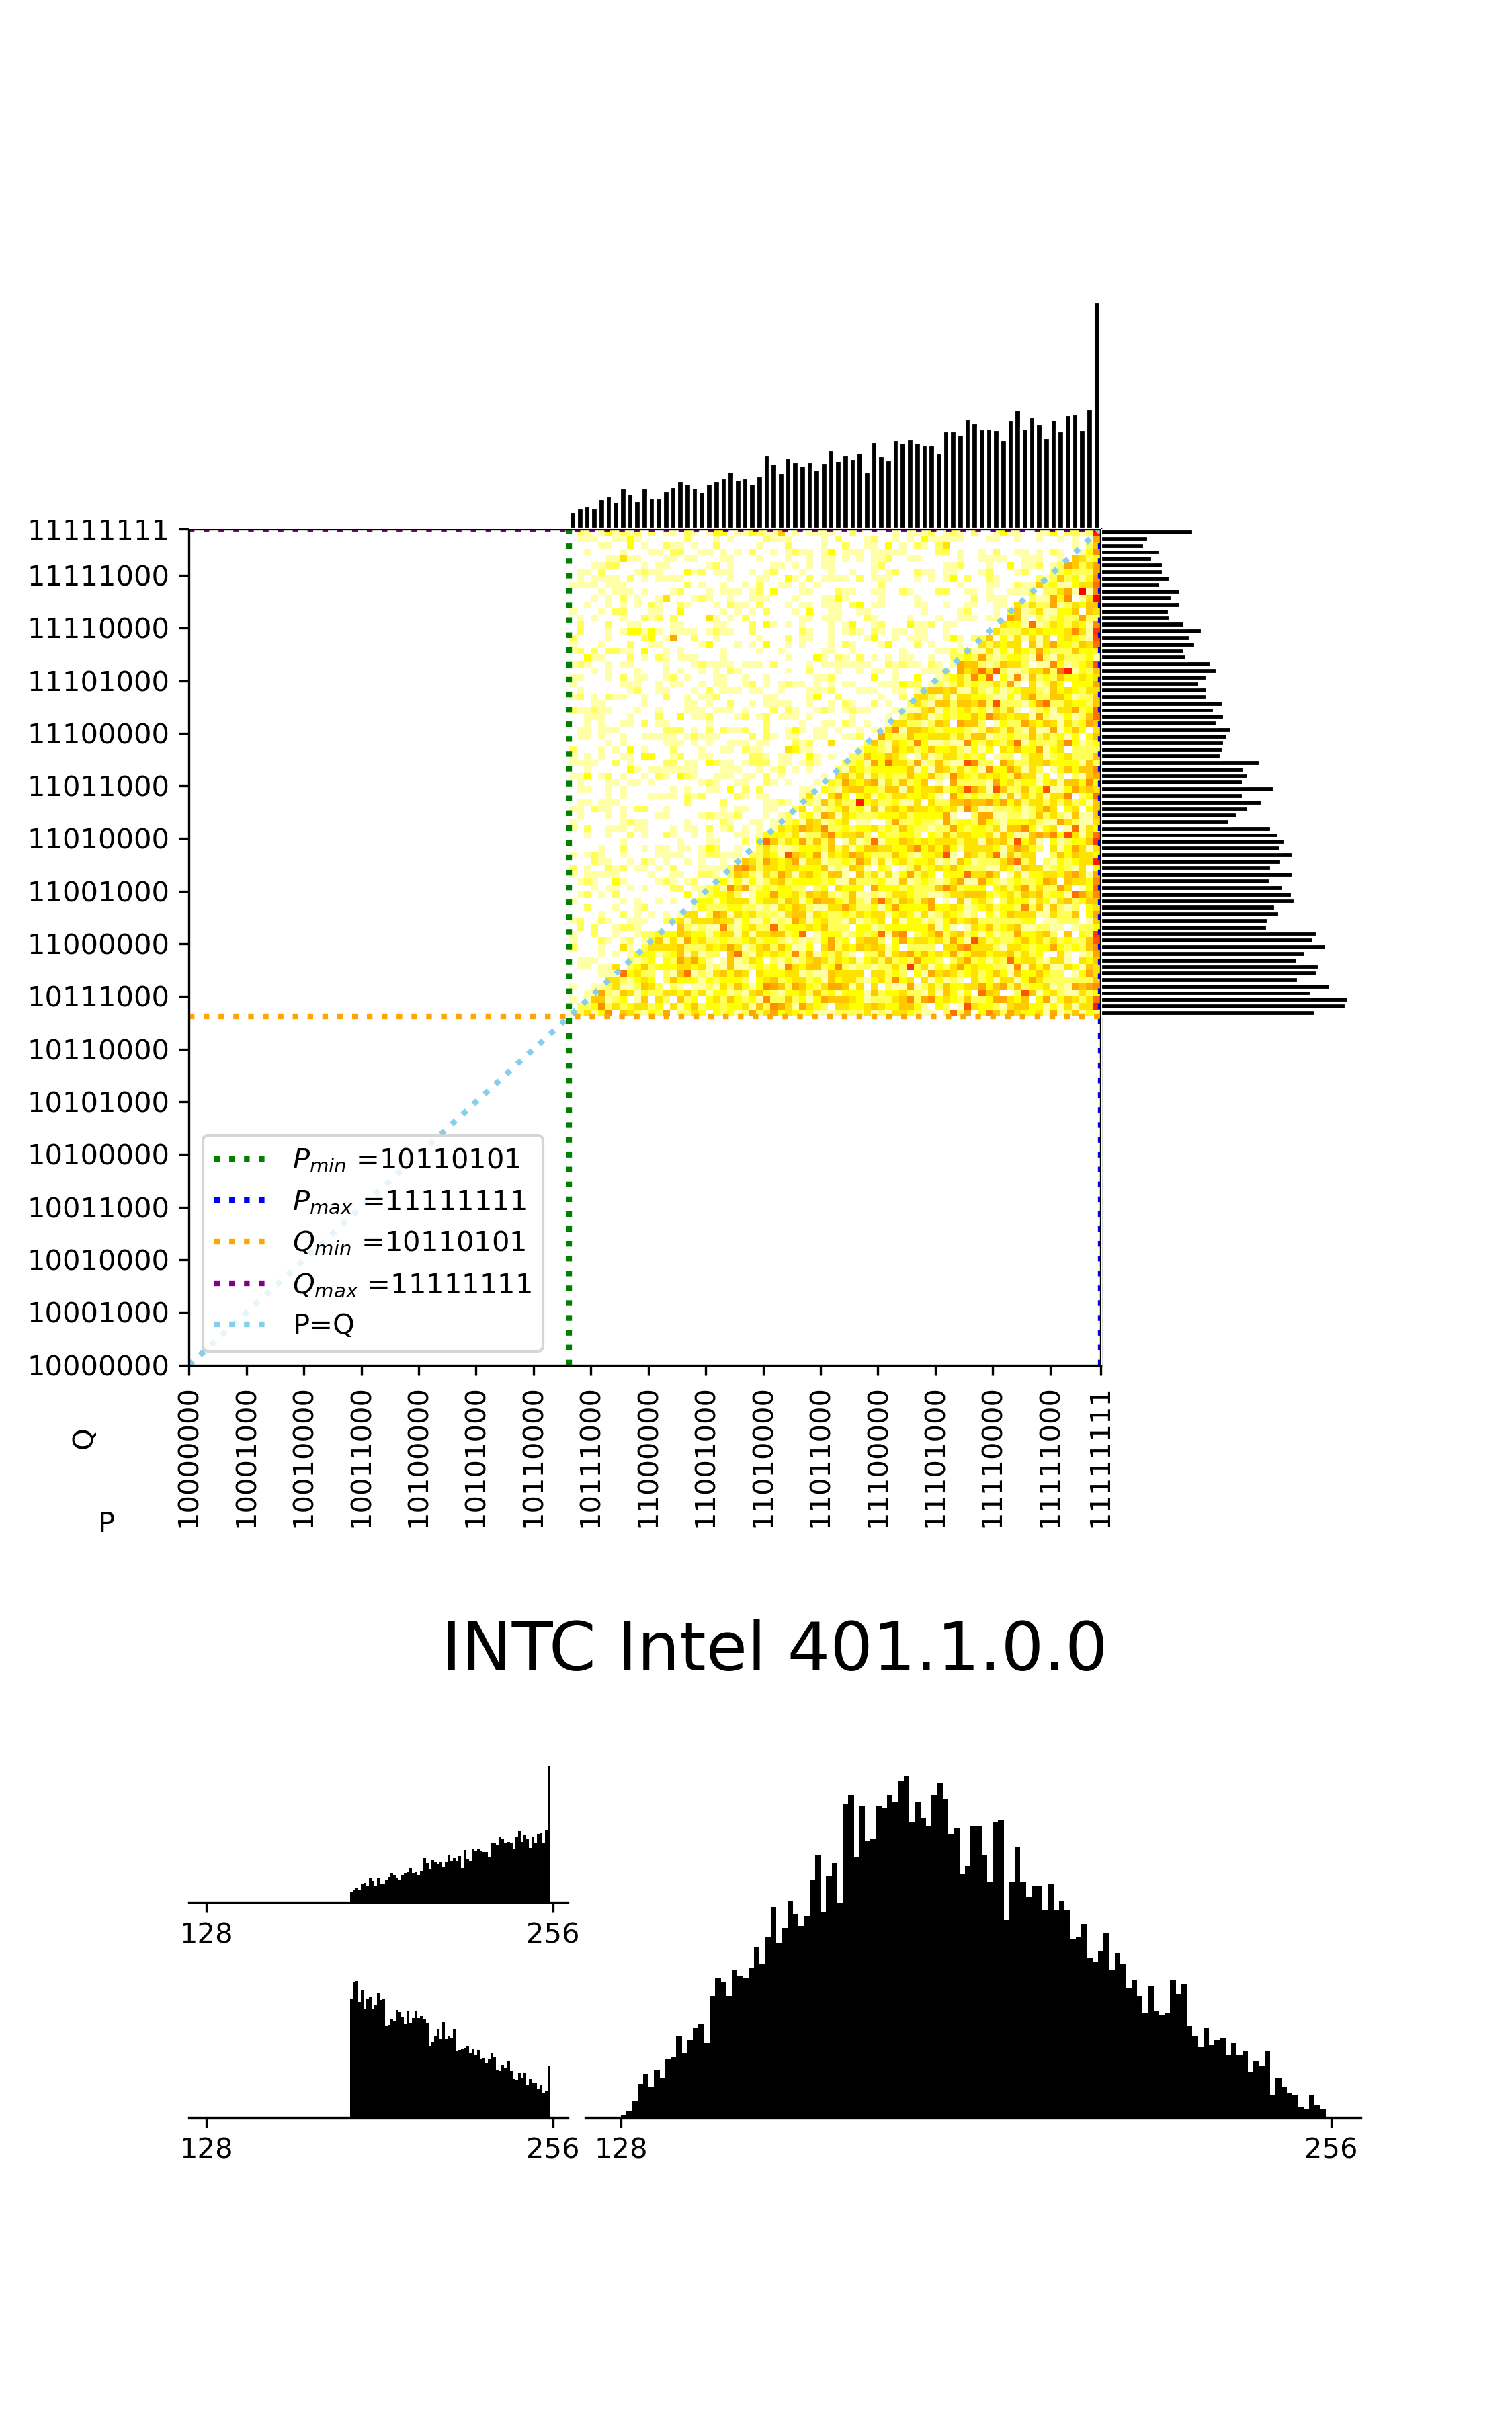
\includegraphics[width=\textwidth,height=\textheight-1.5cm, keepaspectratio]{img/visualizations/rsa.png}
    \caption{TPM chart showing the heatmap and several histograms of most significant bytes of gathered 1024 bit RSA keys.}
    \label{fig:dev-profiles-diagram}
\end{figure}





\renewcommand{\thechapter}{C}
\chapter{Data Attachments}
  \backmatter
  \printindex
  \begingroup
  \sloppy
  \printbibliography
\endgroup


\end{document}

